\chapter{blockchain}\label{sec:blockchain}

Durante la historia de la humanidad, el ser humano siempre ha realizado transacciones entre ellos siendo un tema delicado la confianza en prójimo. Es por ello que se recurren a intermediarios para resolver este problema. Este es el caso de los bancos para actividades financieras, servidores centrales para almacenar datos y computación o incluso gobiernos para mantener la sociedad. La confianza puesta en los intermediarios es asumida: asumimos que van hacer lo que se suponen que tienen que hacer. Sin embargo esto no es así en la práctica. Las máquinas fallan, las personas cometen errores.

En este contexto, surge la tecnología \textit{blockchain}~\cite{duc-2023}. Una tecnología descentralizada en la que no actúa ningún intermediario. La \textit{blockchain} intenta solventar las debilidades del intermediario centralizado en cuatro grandes aspectos: confianza, seguridad, privacidad y transparencia. Mientras que un servidor como único punto de contacto puede ser atacado y los datos almacenados pueden ser alterados de manera maliciosa, esto queda solventado con la \textit{blockchain}.

\section{¿Qué es la \textit{blockchain}?}
Una vez introducida la motivación para la \textit{blockchain} y su potencial, nos centraremos en qué es. Se puede definir de manera informal basándonos en qué nos ofrece: una tecnología para registrar transacciones y procesamiento que es segura (no puede haber ni pérdida ni alteración de los datos) y \textit{trustless} (no hace uso de ningún intermediario en el que confiar). Una definición más completa sería verla como un sistema de computación descentralizada con cinco componentes:
\begin{itemize}
    \item \textbf{Red descentralizada}: la \textit{blockchain} confía en una red descentralizada de ordenadores, llamados nodos, que contribuyen con recursos de computación para ayudar a almacenar y procesar transacciones. Estos ordenadores trabajan de manera autónoma y se comunican mediante una red \ac{P2P}. La mayoría de las redes \textit{blockchain} incluyendo a Bitcoin~\cite{bitcoin} adoptan una topología \ac{P2P} no estructurada, es decir, cada nodo escoge a sus vecinos de manera arbitraria. Otra redes como Ethereum~\cite{ethereum} usan una estructurada. Una topología no estructurada puede ser menos eficiente pero más fácil de mantener.
    \item \textbf{Criptografía}: los métodos de criptografía usados en la \textit{blockchain} dan demostraciones matemáticas de que la \textit{blockchain} debe de funcionar como se supone. Se usan \textit{hashes} criptográficos para vincular bloques de datos en la cadena de forma que no se permita ninguna modificación después de registrarlos en la \textit{blockchain}. Cada transacción se encripta con criptografía de clave pública para asegurar que quien crea la transacción es verificable usando una firma digital y que solo quien se indica como receptor puede recibirla. La confidencialidad de la transacción se logra gracias al uso de \textit{Zero Knowledge Proofs}~\cite{zkp-blockchain}, un mecanismo criptográfico que permite validar la veracidad de una afirmación sin conocer información sensible sobre esta. La elección de la criptografía a usar determina el rendimiento y garantías de la \textit{blockchain}.
    \item \textbf{Registro de transacciones}: Como tecnología de almacenamiento, la \textit{blockchain} es un registro digital que almacena las transacciones en bloques de manera cronológica.
    \item \textbf{Consenso distribuido}: cuando se tiene que tomar alguna decisión, por ejemplo, si una transacción es válida, no hay ninguna autoridad central para decidir. En su lugar, la decisión se hace basándose en un consenso entre los nodos participantes. Por lo tanto, la red \textit{blockchain} debe de tener un protocolo de consenso para asegurarse de que cada transacción o bloque añadido a la \textit{blockchain} es la única opción válida que es aceptada por todos los nodos. La elección del mecanismo de consenso es la decisión más importante a la hora de diseñar una red \textit{blockchain}, por ello más adelante nos centraremos este componente más adelante.
    \item \textbf{\textit{Smart Contracts}}: una \textit{blockchain} se puede ver como un ordenador no convencional que realiza ciertas tareas. En lugar de integrar unidades de procesamiento (CPUs) como un ordenador normal, la \textit{blockchain} es un ordenador descentralizado que usa cientos o miles de ordenadores alrededor del mundo. Las aplicaciones que se ejecutan en la \textit{blockchain} son conocidas como \textit{smart contracts}.
\end{itemize}

\begin{figure}
    \centering
    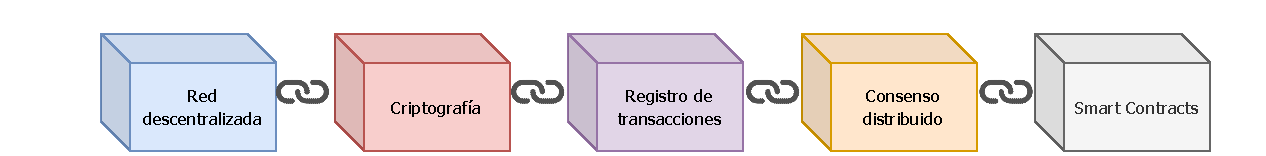
\includegraphics[width=\textwidth]{figuras/blockchain diagram.pdf}
    \caption{Diagrama indicando los 5 componentes de una \textit{blockchain}. Fuente: elaboración propia.}
    \label{fig:blockchaindiag}
\end{figure}

\section{La Estructura de Cadena}
Normalmente, salvo en casos poco populares, el registro de la \textit{blockchain} sigue una estructura de cadena~\cite{survey-blockchain}. Los datos están organizados en bloques de datos: $\{b_1, b_2, \dots\}$. Cuando se necesita almacenar nuevas transacciones, estas se colocan en un nuevo bloque que se añadirá después del último bloque ya existente de la cadena. Además de almacenar la información de la transacción, el estado de la \textit{blockchain} si procede, e información necesaria en una cabecera, el bloque tiene dos atributos fundamentales:
\begin{itemize}
    \item \textbf{ID del bloque}: este es el \textit{hash} del contenido del bloque usando una función de \textit{hash} criptográfica $H$. Esta función está predefinida y se conoce de manera pública.
    \item \textbf{El hash anterior}: es el ID del bloque anterior.
\end{itemize}

Notemos que el ID del bloque no tiene por qué ser necesariamente almacenado en el bloque ya que se puede calcular a partir del contenido del bloque.

El \textit{hash} anterior es una información crítica para mantener la integridad de la cadena. Si cualquier parte de cualquier bloque cambiase después de registrarse en la \textit{blockchain}, este cambio será detectado. Esto es porque para añadir un nuevo bloque a la \textit{blockchain} se debe de cumplir un proceso llamado validación del bloque~\cite{duc-2023}. Un nuevo bloque $b_{i+1}$ es válido si:
\begin{enumerate}
    \item El \textit{hash} anterior es consistente, esto es: $b_{i+1}^{prev} = H(b_i)$.
    \item Todas las transacciones de $b_{i+1}$ son válidas.
    \item El bloque $b_i$ es válido.
\end{enumerate}

La verificación en el paso 1 necesita calcular el \textit{hash} de $b_i$ y compararlo con $b_{i+1}^{prev}$. El paso 3 necesita ejecutar el mismo proceso de validación para verificar la validez del bloque $b_i$. Consecuentemente, para validar el bloque $b_{i+1}$, se necesita comprobar todos los \textit{hash} anteriores de todos los bloques $b_j$ con $j \le i+1$. Si un bloque anterior, digamos, $b_{j-1}$ ha sido modificado, entonces cuando calculemos su \textit{hash}, $H(b_{j-1})$, encontraremos que es distinto del valor $b_j^{prev}$ almacenado en el bloque $b_j$. Esto resulta en una infracción y como resultado el nuevo bloque $b_{i+1}$ se considerará inválido y no se añadirá a la \textit{blockchain}.

Una consecuencia de haber modificado el bloque $b_j$ es que la \textit{blockchain} no podrá crecer más. Uno podría pensar que en ese caso la \textit{blockchain} se vuelve inútil ya que detiene a toda la \textit{blockchain}. Esto sería cierto si la red \textit{blockchain} estuviese compuesta de un único ordenador. En la práctica, la red \textit{blockchain} está compuesta de varios ordenadores~\cite{duc-2023}, donde los datos de la \textit{blockchain} están duplicados en cada nodo. Para que un nodo se asegure de que su copia de la \textit{blockchain} es correcta, necesita comparar su copia con la de sus vecinos para escoger la \textit{blockchain} más larga como la correcta~\cite{bitcoin}. Antes de realizar esta comparación, el nodo necesita verificar la validez de la copia de cada vecino, lo que implica validar todos los bloques de la copia. Por lo tanto, si la copia de la \textit{blockchain} de algún nodo incluye alguna infracción, esta copia no será considerada válida. Por lo tanto, los nodos honestos de la red nunca usarán una copia errónea~\cite{bitcoin}.

\section{Cómo Conseguir un Consenso}

El consenso ya era un área de investigación en computación con 30 años de estudio antes de que la tecnología \textit{blockchain} se volviese popular. Comenzó en los años 70 con el proyecto de la NASA, ``\textit{Software Implemented Fault Tolerance} (SIFT)``~\cite{sift}, enfocado a construir un sistema de control de naves resistente. El reto consistía en replicar el sistema en múltiples máquinas de manera que el sistema se pudiese resistir fallos de múltiples de ellas. Más adelante este reto se formuló como el ahora conocido ``Problema de los Generales Bizantinos``~\cite{byzantine-general}. Este problema popularizó el término ``Fallo Bizantino (\textit{Byzantine Fault})`` para indicar una condición de un sistema distribuido donde algunos nodos no son confiables y pueden aparentar normales o maliciosos de manera arbitraria, pudiendo camuflarse entre ellos de manera que no haya información consistente para que los otros nodos declaren su mal funcionamiento.

Un sistema sistema \ac{BFT}~\cite{sift} debe de evitar el fallo completo y por tanto los nodos deben de acordar una estrategia común y seguir este consenso, sabiendo que algunos nodos pueden fallar o actuar de manera maliciosa. Para describir \ac{BFT} de manera formal, consideremos un sistema de difusión donde un nodo necesita difundir un mensaje (valor) a todos los demás nodos de manera par a par. Al principio, en nodo emisor recibe un valor de entrada $m$. El protocolo de difusión debe concluir con que cada nodo $i$ tenga un valor de salida $m_i$. El emisor y los receptores pueden ser honestos o deshonestos. Este protocolo logra \ac{BFT} si cumple dos requisitos:
\begin{itemize}
    \item \textbf{Consistencia}: todos los nodos honestos $i$ y $j$ deben de tener el mismo valor: $m_i=m_j$.
    \item \textbf{Validez}: si el emisor es honesto, todos los nodos honestos $i$ deben de tener el mismo valor: $m=m_i$.
\end{itemize}

Un sistema puede ser consistente pero no válido, cuando todos los nodos honestos tienen el mismo valor de salida pero no es el mismo que el del emisor. Un sistema puede ser válido pero no consistente, cuando el emisor no es honesto y transmite valores distintos a los nodos. Por tanto, ninguno de los requisitos es condición suficiente.

Una \textit{blockchain} es un sistema \ac{BFT}. Para solventar las inconsistencias debido al trabajo autónomo e independiente de los nodos, la solución estándar es que cada nodo esté de acuerdo en que la copia más larga de la \textit{blockchain}, es decir, la que tiene más bloques, es la versión globalmente correcta. Debido a que las copias más cortas que la correcta no se usan, los nodos quieren tener sus copias lo más actualizadas posibles ya que si no podrían malgastar esfuerzos en añadir bloques a la \textit{blockchain} equivocada. Como consecuencia, aunque a veces algunas transacciones sean registradas en distintas copias de la \textit{blockchain} en nodos distintos, varias transacciones pueden ser añadidos al último bloque de la \textit{blockchain} existente en distintos nodos, o aunque distintos nodos pueden tener copias distintas de la \textit{blockchain}, al final estos nodos tendrán la misma copia de la \textit{blockchain}.

Sin embargo esto es solo en teoría. Si un consenso ocurre demasiado tarde, las inconsistencias mencionadas previamente causarán que el sistema rinda de manera incorrecta. Por lo tanto, necesitamos minimizar la probabilidad de estas inconsistencias y minimizar el tiempo que se tarda en alcanzar el consenso de la \textit{blockchain}. Para esto, se han usado distintos mecanismos de consenso en \textit{blockchain}. Entre los más comunes están la \ac{PoW} o la \ac{PoS}.

\section{Algoritmos de Consenso}
Para hacer una comunicación confiable entre los nodos y mantener el estado correcto a través del sistema incluso en presencia de nodos maliciosos o incluso ante fallos de la red, se usan los conocidos algoritmos de consenso brevemente expuestos anteriormente. El algoritmo de consenso es el responsable para mantener copias consistentes del estado actual de la \textit{blockchain} en todos los nodos, validar nuevas transacciones y actualizar el estado actual mientras se alcanza un acuerdo entre los nodos. Nos centraremos en explicar los dos algoritmos de consenso más populares, \ac{PoW} y \ac{PoS}.
\subsection{Proof Of Work}
El algoritmo de \ac{PoW} normalmente necesita un nodo de prueba y otro de verificación. El nodo de prueba realiza una tarea computacionalmente intensiva para encontrar una solución a un problema de una cierta dificultad. El resultado entonces se presenta al verificador que consume significantemente menos recursos para verificar el resultado. La asimetría y la excesiva cantidad de recursos necesitados por el nodo de prueba sirve para lograr dos propósitos:
\begin{enumerate}
    \item Mitiga ataques sibilinos a nivel de consenso. Lanzar un ataque sibilino necesita a un adversario creando múltiples entidades maliciosas o a varias entidades coordinadas entre sí. Sin embargo, por diseño, la cantidad de recursos computacionales es importante para el algoritmo de \ac{PoW}, no la cantidad de nodos.
    \item La carga de trabajo en sí se convierte en un seguro contra ataques de bifurcación. La longitud de la cadena es prácticamente proporcional a la cantidad de recursos gastados minando bloques. Si el adversario quiere modificar una transacción del pasado, necesita primero tener más del 51\% de los recursos computacionales dentro de la red, bifurcar una nueva cadena a partir del bloque objetivo, y minar los bloques hasta que la nueva cadena se vuelva la más larga.
\end{enumerate}

Normalmente los algoritmos de \ac{PoW} emplean tareas que computacionales que hacen uso de la CPU o de la GPU. La red más famosa que usa este tipo de algoritmo es la de Bitcoin. El algoritmo necesita encontrar un número llamado \textit{nonce} tal que, cuando es \textit{hasheado} con los contenidos del bloque (usando SHA-256d, esto es, SHA-256 aplicado dos veces), el resultado sea un número menor que un valor de dificultad. Cuando un \textit{nonce} adecuado se encuentra y es aprobado por los verificadores, el nodo que lo ha encontrado obtiene una recompensa. El proceso de encontrar este número se llama minar, y a los nodos que lo buscan se llaman mineros.

\subsection{Proof Of Stake}
Para solventar las desventajas de algoritmos de \ac{PoW} tales como minado centralizado y consumo energético, los algoritmos de \ac{PoS} están ganando fuerza. Un algoritmo de \ac{PoS} intenta validar transacciones y logra consenso en la red sin el uso de tareas computacionalmente intensas. En lugar de ``trabajar``, un nodo verificador tiene que bloquear su ``participación``, que es una parte de su riqueza en la red.

En un algoritmo de \ac{PoS}, los propietarios de la participación bloquean su ``participación`` y se vuelven elegibles para participar en la validación de la transacción y en la creación de un nuevo bloque. Estos no minan nuevas monedas a diferencia de los algoritmos de \ac{PoW}. En su lugar, recolectan las tasas de transacción o intereses proporcionales a su participación como recompensa. Si el nodo se identifica como malicioso, su participación y recompensa pueden ser confiscadas, lo que sirve como un aliciente económico para evitar nodos maliciosos.

Las ventajas de un algoritmo de \ac{PoS} sobre uno de \ac{PoW} son las siguientes:
\begin{itemize}
    \item \textbf{Descentralización}: en los algoritmos de \ac{PoW} los mineros pueden tener un incremento exponencial en recursos computacionales cuando se invierte en equipamiento centrado en el minado. En una red de \ac{PoS}, la ganancia es directamente proporcional a la cantidad de participación que el nodo decide invertir.
    \item \textbf{Eficiencia energética}: los algoritmos de \ac{PoW} consumen mucha energía. En el caso de Bitcoin, sus mineros consumen más energía que países como Portugal, Singapur o la República Checa. Los algoritmos de \ac{PoS} no necesitan que los nodos resuelvan tareas computacionalmente intensas cuando se crean nuevos bloques. Por lo tanto pueden ser altamente eficientes a nivel energético.
\end{itemize}